% arara: pdflatex
% font size
\documentclass[a4paper,11pt]{article}
\usepackage[T1]{fontenc} 
\usepackage[utf8]{inputenc}
% language
\usepackage[english]{babel}

\usepackage{graphicx}
\usepackage{ragged2e}

\usepackage[format=plain,justification=RaggedRight,singlelinecheck=false,font={small},labelsep=space]{caption}
\usepackage[dvipsnames]{xcolor}	
\usepackage[a4paper]{geometry}
    % border size
    % left 3.5 right 2.5 for printing with binding
	\geometry{left=3cm,right=3cm,top=2.4cm,bottom=2cm}
	% row spacing
	\usepackage[onehalfspacing]{setspace}
	\renewcommand{\\}{\vspace*{0.5\baselineskip} \newline}
\renewcommand*\MakeUppercase[1]{#1}	
\usepackage{fancyhdr}
	\pagestyle{fancy}
	\renewcommand{\headrulewidth}{0pt}
	\renewcommand{\footrulewidth}{0pt}
	\fancyhead[R]{\footnotesize{\thepage}}
	\fancyhead[L]{\footnotesize{\leftmark}}
	\fancyfoot{}
\usepackage[colorlinks,
pdfpagelabels,
pdfstartview = FitH,
bookmarksopen = true,
bookmarksnumbered = true,
linkcolor = black,
urlcolor = cyan,
plainpages = false,
hypertexnames = false,
citecolor = black,
colorlinks=true] {hyperref}
\usepackage{import}
% syntax highlighting
\usepackage{minted}

\usepackage{listings}

% TODO define langauge
\lstdefinelanguage{conf}{}

% START CODE STYLING YAML
\newcommand\YAMLcolonstyle{\color{red}\mdseries}
\newcommand\YAMLkeystyle{\color{black}\bfseries}
\newcommand\YAMLvaluestyle{\color{blue}\mdseries}

\makeatletter

% here is a macro expanding to the name of the language
% (handy if you decide to change it further down the road)
\newcommand\language@yaml{yaml}

\expandafter\expandafter\expandafter\lstdefinelanguage
\expandafter{\language@yaml}
{
  keywords={true,false,null,y,n},
  keywordstyle=\color{darkgray}\bfseries,
  basicstyle=\YAMLkeystyle,                                 % assuming a key comes first
  sensitive=false,
  comment=[l]{\#},
  morecomment=[s]{/*}{*/},
  commentstyle=\color{purple}\ttfamily,
  stringstyle=\YAMLvaluestyle\ttfamily,
  moredelim=[l][\color{orange}]{\&},
  moredelim=[l][\color{magenta}]{*},
  moredelim=**[il][\YAMLcolonstyle{:}\YAMLvaluestyle]{:},   % switch to value style at :
  morestring=[b]',
  morestring=[b]",
  literate =    {---}{{\ProcessThreeDashes}}3
                {>}{{\textcolor{red}\textgreater}}1     
                {|}{{\textcolor{red}\textbar}}1 
                {\ -\ }{{\mdseries\ -\ }}3,
}

% switch to key style at EOL
\lst@AddToHook{EveryLine}{\ifx\lst@language\language@yaml\YAMLkeystyle\fi}
\makeatother

\newcommand\ProcessThreeDashes{\llap{\color{cyan}\mdseries-{-}-}}
% END CODE STYLING YAML

\begin{document}
\import{other/}{title}

\pagenumbering{Roman}

\tableofcontents\newpage
%\listoftables\addcontentsline{toc}{section}{List of Tables}\newpage

\pagenumbering{arabic}

\section{Introduction}
The practical phase took place in the setting of an Internet of Things "Smart Building" project. Smart Building is a showcase project since inovex GmbH is also the customer. Gathering knowledge for potential external customer projects is an important objective beside finishing the project. That said, sometimes a solution seems to be over-engineered for our business case but is designed for a larg scale customer project.

\subsection{Company}
"Inovex is an IT project centre driven by innovation and quality, focusing its services on "Digital Transformation". The main three subdivisions are "Application Development", "Data Management \& Analytics" and "IT Engineering \& Operations" in which I work in the scope of this project.\\
"IT Engineering and Operations" handles the combined disciplines required for the flexible, reliable operation of systems in data centres: the design, installation and configuration of server infrastructures, and the daily maintenance and running of these systems. The focus is on high availability and scalability, migrations, the cloud, and open-source data centre management."\cite{inovex}

\subsubsection{Philosophy}
"Here at inovex, we are using an iterative strategy process to manage our own agile transformation. We also believe in flat hierarchies, and we base all our decisions on agile values.\\
As all our project teams are self-organised and agile skills are, therefore, essential, every new inovex employee receives training in agile methods. We also support our employees by holding meetings in agile formats (like Lean Coffee) and by facilitating the internal transfer of knowledge (through brown bag lunches and tech days, for example).\\
Many of our internal teams work agilely and thus enjoy a high level of transparency, quality and efficiency. Our Marketing Team, HR Team and Sales Team have each established different agile methods tailored specifically to their requirements and they use these in combination with our ISO-certified quality management processes."\cite{inovex}
\newpage

\subsection{Internet of Things}
Internet of Things "is the concept of basically connecting any device with an on and off switch to [a network]. This includes everything from cellphones, coffee makers, washing machines, headphones, lamps [to] wearable devices ... .\\
This also applies to components of machines, for example a jet engine of an airplane or the drill of an oil rig."\cite{forbes-iot}

\subsection{Smart Building}
"Smart Building" is the digitization of an entire construction. This includes automating, controlling and linking every technical device inside the building. The purpose is to manage these devices more intelligently to reduce energy costs or lower the carbon footprint.\cite{kiwi-sb}\\
A popular example is a light that automatically turns on if a person enters the corridor and turns off after it stops detecting movements. A more complex scenario would be windows that open and close depending on the CO2 saturation in the room.
\newpage

\section{Project}
Inovex has seven locations with five to ten meeting rooms each. These can be added to any appointment in Google Calendar so they are blocked for the duration of this event.\\
Long-term projects have multiple reoccurring meetings with rooms assigned, so people from corresponding offices are always able to have a quiet and collaborative place for the event. Since every inovex employee can decide if they want to work from home and join the meeting remotely, there are plenty of meeting rooms falsely occupied if participants decide to stay at home.\\
This leads to joining spontaneous meetings from open workspaces because all meeting rooms are blocked even though some might be available. Coworkers in the same workspace can get distracted.\\
Smart meeting rooms should determine their real status and unblock if necessary.

\subsection{Mender}
"Mender is an open source over-the-air (OTA) software updater for embedded Linux devices. Mender comprises a client running at the embedded device, as well as a server that manages deployments across many devices. ...\\
Robustness is ensured with atomic image-based deployments using a dual A/B rootfs partition layout. This makes it always possible to roll back to a working state, even when losing power at any time during the update process. ...\\
Mender not only provides the client-side updater, but also the backend and UI for managing deployments as open source. The Mender server is designed as a microservices architecture and comprises several repositories."\cite{mender-github}

\subsection{Mender Integration Server}
Modern applications are often built with a microservice architecture. This structures the application to be a collection of highly maintainable individual services, which are loosely coupled and independently deployed.\cite{microservicesio}\\
The Mender Integration Server, also referred to as Mender Hub, consists of twelve services. Unless microservices, some of them depend on each other on startup.\\
The application exposes an API-Gateway and a Storage-Proxy for users to interact with. They are proxies to other internal services.\cite{mender-github}\\
Figure \ref{fig:mender-integration} shows all microservices and their network connections.
\begin{figure}
    \centering
    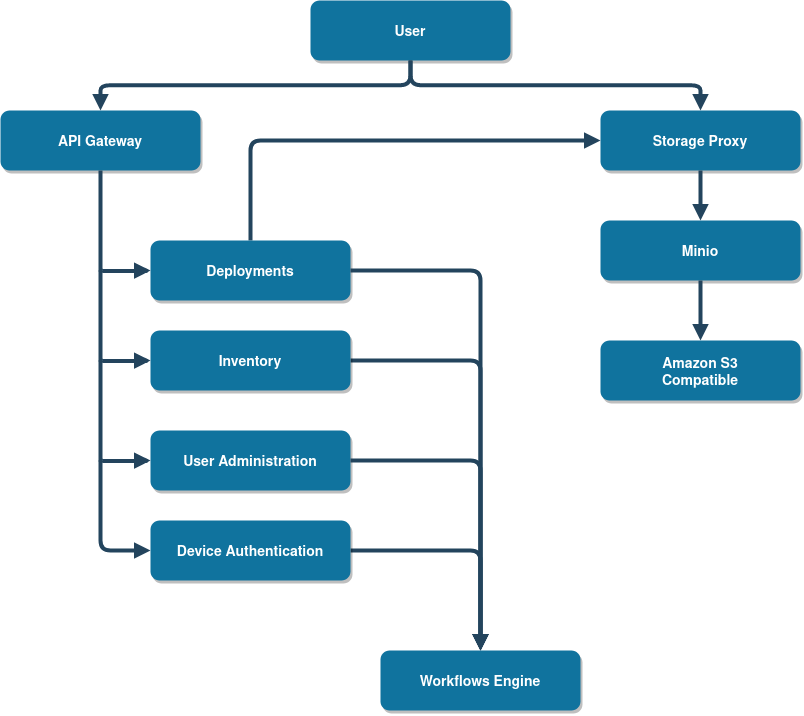
\includegraphics[scale=0.5]{images/integration-app.png}
    \caption{Mender Integration Server Architecture}
    \label{fig:mender-integration}
\end{figure}
Minio is a third-party object storage. It can either be used to serve uploaded content on its own or proxy requests to Amazon S3 compatible cloud providers. All other services are mender application logic web services.

\subsubsection{Docker-Compose} \label{docker-compose}
Compose is a tool for defining and running multi-container Docker applications. With Compose, a YAML file is used to configure the applications services. Then, with a single command, all services from the configuration are created and started.\cite{docker-compose}\\
Compose runs on a single machine. To distribute services across multiple nodes, the creators of Docker-Compose introduced Docker-Swarm. This tool is not as feature-rich as Compose and requires YAML configuration file changes in order to run Docker-Compose files with Docker-Swarm.\\
The Mender Integration Server uses Docker-Compose to define their application stack. This allows users a simple and quick local production or development setup on a single machine.\\
Container orchestration platforms are used to scale containerized applications like Mender Integration Server on higher load. Common platforms are Kubernetes, Nomand or Apache Mesos. These tools allow users to ship their containers to a platform which distributes them to any node on the cluster. This enables higher workload for large scale applications because it can be distributed to different compute nodes.\\
A scaleable Mender Hub is important for potential customers which want to handle multiple thousand IoT devices at a time. Critical updates need to be delivered quickly. Handling a batch of devices after another is often not an option.
\begin{code}
  \captionof{listing}{Original Docker-Compose YAML}
  \label{org-dc}
  \begin{minted}{yaml}
version: '2.1'
services:

  mender-deployments:
    command: server --automigrate
    image: mendersoftware/deployments:mender-2.4.0
    restart: on-failure
    volumes:
      - ./storage.crt:/etc/ssl/certs/storage-proxy.crt
    environment:
      STORAGE_BACKEND_CERT: /etc/ssl/certs/storage-proxy.crt
      DEPLOYMENTS_AWS_AUTH_KEY: minio
      DEPLOYMENTS_AWS_AUTH_SECRET: minio123
      DEPLOYMENTS_AWS_URI: https://storage-proxy:9000
    networks:
      - mender
    depends_on:
      - mender-mongo
      - storage-proxy

  mender-gui:
    image: mendersoftware/gui:mender-2.4.0
    restart: on-failure
    networks:
      - mender
    environment:
      - GATEWAY_IP
      - INTEGRATION_VERSION
      - MENDER_ARTIFACT_VERSION
      - MENDER_VERSION
      - MENDER_DEB_PACKAGE_VERSION

  mender-api-gateway:
    image: mendersoftware/api-gateway:mender-2.4.0
    restart: on-failure
    ports:
      - 443:443
    volumes:
      - ./gateway.crt:/var/www/mendersoftware/cert/cert.crt
      - ./gateway.key:/var/www/mendersoftware/cert/private.key
    environment:
      ALLOWED_HOSTS: localhost
      HSTS_MAX_AGE: 0
    networks:
      - mender
    depends_on:
      - mender-device-auth
      - mender-deployments
      - mender-gui
      - mender-useradm
      - mender-inventory

  mender-device-auth:
    command: server --automigrate
    image: mendersoftware/deviceauth:mender-2.4.0
    restart: on-failure
    volumes:
      - ./deviceauth.key:/etc/deviceauth/rsa/private.pem
    environment:
      DEVICEAUTH_ORCHESTRATOR_ADDR: >-
        http://mender-workflows-server:8080/
    networks:
      - mender
    depends_on:
      - mender-mongo
      - mender-workflows-server

  mender-inventory:
    command: server --automigrate
    image: mendersoftware/inventory:mender-2.4.0
    restart: on-failure
    networks:
      - mender
    depends_on:
      - mender-mongo

  mender-useradm:
    command: server --automigrate
    image: mendersoftware/useradm:mender-2.4.0
    restart: on-failure
    volumes:
      - ./useradm.key:/etc/useradm/rsa/private.pem
    networks:
      - mender
    depends_on:
      - mender-mongo

  mender-workflows-worker:
    image: mendersoftware/workflows-worker:mender-2.4.0
    restart: on-failure
    command: >-
      worker
      --automigrate
      --excluded-workflows
      generate_artifact
    environment:
      WORKFLOWS_MONGO_URL: mongodb://mender-mongo:27017
    networks:
      - mender
    depends_on:
      - mender-mongo

  mender-create-artifact-worker:
    command: --automigrate
    image: mendersoftware/create-artifact-worker:mender-2.4.0
    restart: on-failure
    environment:
      - CREATE_ARTIFACT_SKIPVERIFY=1
      - WORKFLOWS_MONGO_URL=
          mongodb://mongo-workflows:27017
      - CREATE_ARTIFACT_GATEWAY_URL=
          https://mender-api-gateway
      - CREATE_ARTIFACT_DEPLOYMENTS_URL=
          http://mender-deployments:8080
    networks:
      - mender
    depends_on:
      - mender-mongo

  mender-mongo:
    image: mongo:3.6
    restart: on-failure
    networks:
      mender:
        aliases:
          - mongo-deployments
          - mongo-device-auth
          - mongo-inventory
          - mongo-useradm
          - mongo-workflows

  minio:
    image: minio/minio:RELEASE.2018-09-25T21-34-43Z
    restart: on-failure
    command: server /export
    environment:
      MINIO_HTTP_TRACE: /dev/stdout
      MINIO_ACCESS_KEY: minio
      MINIO_SECRET_KEY: minio123
    networks:
      mender:
        aliases:
          - minio.s3.docker.mender.io

  storage-proxy:
    image: openresty/openresty:1.13.6.2-0-alpine
    restart: on-failure
    ports:
      - 9000:9000
    volumes:
      - ./storage.crt:/var/www/storage-proxy/cert/cert.crt
      - ./storage.key:/var/www/storage-proxy/cert/private.key
    networks:
      mender:
        aliases:
          - s3.docker.mender.io
    depends_on:
      minio:
        condition: service_healthy


networks:
  mender:
  \end{minted}
\end{code}
Listing \ref{org-dc} shows a YAML configuration to run Mender Hub via Docker-Compose on a local machine.

\subsection{Yocto}
"The Yocto Project (YP) is an open source collaboration project that helps developers create custom Linux-based systems regardless of the hardware architecture.\\
The project provides a flexible set of tools and a space where embedded developers worldwide can share technologies, software stacks, configurations, and best practices that can be used to create tailored Linux images for embedded and IoT devices, or anywhere a customized Linux OS is needed."\cite{yoctoproject}\\
Popular distributions like Ubuntu Server ship with plenty of nice features, services and tools. IoT devices are dedicated to do a specific task. Many features of these generalised distributions are therefore not needed in IoT environments. Creating a minimal distribution with Yocto increases performance, battery life and free disk space.\\
Mender Software maintains an official Yocto recipe which adds the Mender client to an image. This client connects the device to Mender Hub and enables over the air (OTA) updates. Community driven Yocto example setups for most popular micro controllers like Raspberry Pi, Asus Tinkerboard or Intel NUC are available on the Mender Forums.

\section{Prerequisites}
\subsection{Transport Layer Security}
The official Docker-Compose Mender setup wants users to mount an SSL certificate to the API-Gateway and Storage-Proxy. This should prevent unsecured Mender Hub servers on the internet. The SSL termination in production setups is often handled by third party services like Certbot. These services automatically generate certificates before they expire and make use of a reverse proxy to expose a secured endpoint to users.\\
A reverse proxy terminates incoming connections, opens a new connection to the desired destination and route all traffic as if the proxy server would be the desired destination server. Proxy and destination server can communicate unsecured via HTTP if they are in the same private network. The user communicates secured via SSL with the reverse proxy server. This setup reduces overhead for deploying applications, because developers do not have to implement encrypted communication.\\
Mender has no official way to deactivate SSL termination in the API-Gateway and Storage-Proxy. The API-Gateway consists of a Nginx webserver which proxies all requests to corresponding services inside the network. The gateways source code is public available on Github: \href{https://github.com/mendersoftware/mender-api-gateway-docker}{mendersoftware/mender-api-gateway-docker}. In order to have changes done in scope of the practical phase merged upstream, it is recommended to avoid breaking changes. SSL should be deactivated via environment variable and stay enabled by default.\\
First step was modifying the original \verb|nginx.conf| file to only expose port 80 and remove all SSL specific configuration. The \verb|include| statement in Nginx allows reusing parts of your configuration file in multiple different files. After extracting all common configuration into a separate config file, the entrypoint script needs to decide whether to use \verb|nginx.ssl.conf| or \verb|nginx.no-ssl.conf| as \verb|nginx.conf| based on the environment variable \verb|SSL|. This ensures that no duplicated code has to be maintained in the future.\\
The pull request with all changes was merged in the master branch as shown on \href{https://github.com/mendersoftware/mender-api-gateway-docker/pull/109}{Github}.\\

\begin{code}
  \captionof{listing}{nginx.no-ssl.conf}
  \begin{minted}{nginx}
server {
  listen 80;
  # @ALLOWED_HOSTS@ gets changed by the entrypoint
  server_name @ALLOWED_HOSTS@;
  # import application specific configuration
  include /usr/local/openresty/nginx/conf/common.nginx.conf;
}
  \end{minted}
\end{code}
\begin{code}
  \captionof{listing}{nginx.ssl.conf}
  \begin{minted}{nginx}
# redirect http to https
server {
  listen 80;
  # _ is a wildcard and matches every server name
  server_name _;
  return 301 https://$http_host$request_uri;
}

server {
  listen 443 ssl;
  # @ALLOWED_HOSTS@ gets changed by the entrypoint
  server_name @ALLOWED_HOSTS@;

  ssl_certificate /var/www/mendersoftware/cert/cert.crt;
  ssl_certificate_key /var/www/mendersoftware/cert/private.key;

  ssl_protocols TLSv1.1 TLSv1.2;
  ssl_ciphers HIGH:!aNULL:!MD5:!SHA;
  ssl_prefer_server_ciphers on;
  ssl_session_cache shared:SSL:10m;
  ssl_session_tickets off;
  ssl_stapling on;
  ssl_stapling_verify on;
  ssl_trusted_certificate /var/www/mendersoftware/cert/cert.crt;

  add_header Strict-Transport-Security
    "max-age=@HSTS_MAX_AGE@; includeSubdomains; preload";

  # import application specific configuration
  include /usr/local/openresty/nginx/conf/common.nginx.conf;
}
  \end{minted}
\end{code}
\begin{code}
  \captionof{listing}{entrypoint.sh}
  \label{entrypointsh}
  \begin{minted}{bash}
#!/bin/sh

# default is true
SSL=${SSL:-true}

SERVER_BLOCKS_FILENAME="non-ssl"

if [ "$SSL" = "true" ] || [ "$SSL" = "TRUE" ] || [ "$SSL" = "1" ]; then
   CERT_PATH=/var/www/mendersoftware/cert/cert.crt
   KEY_PATH=/var/www/mendersoftware/cert/private.key
   waserr=0

   for f in $CERT_PATH $KEY_PATH; do
       if ! test -e $f; then
           echo "required file $f not found in container"
           waserr=1
       fi
   done

   if [ "$waserr" = "1" ]; then
      echo "certificate or key not found, exiting"
      exit 1
   fi

   SERVER_BLOCKS_FILENAME="ssl"
fi

sed -i -e \
"s/[@]INCLUDE_SERVER_BLOCKS[@]/include 
\/usr\/local\/openresty\/nginx\/conf\/
nginx.$SERVER_BLOCKS_FILENAME.conf;/" \
/usr/local/openresty/nginx/conf/nginx.conf
  \end{minted}
\end{code}
Listing \ref{entrypointsh} includes the correct \verb|nginx.conf| according to the environment variable \verb|SSL| in the main nginx configuration file via \verb|sed| command.

\subsection{Static Configuration}
Mounting files in platforms like Kubernetes is not the recommended way of modifying a container. The problem is that mounted files need to be present on all nodes in the same location. Environment variables on the other hand can be set in Kubernetes YAML files to dynamically distribute to all nodes spawning a certain container. This does not require a specific file structure on host nodes.\\
Another option is to create a YAML string containing the configuration file and pipe this string into a file on container start. These strings cannot be read from the local filesystem as plain text because they are embedded in a YAML key-value pair. If this content should be used in different places, for example in a Docker-Compose development setup, this technique creates duplicated code. The content has to be stored as a YAML key-value pair and a plain text file on the local filesystem.\\
The last option is to bake the configuration file into a custom image and publish it on a private or public registry. If all nodes got access to this registry, kubernetes can pull the image and start containers with all configuration files baked in. Changing the files in this process is slower compared to other techniques. It requires to build and publish a new version of the image. This new version needs to be set in Kubernetes YAML files aswell.\\
In scope of the Smart Building project we decided to statically bake the configuration files into custom images and push them to the inovex Gitlab registry.

\subsection{Persistent Storage}
Folder and file mounts from host operating systems are not problematic in Docker-Compose because it only runs on a single machine. If a service with a folder mount gets restarted, it is guaranteed that the same folder on the same host gets mounted into this service again. Since a Kubernetes cluster consists of many different nodes, the restarted service might start on another node than before. Data written to the folder mount on the old node cannot be mounted to the same container again.\\
Minio and MongoDB are the only Mender services with persistent storage. When using Minio as a storage proxy to Azure, its folder mount can be removed. All files will be stored in the proxied location. Microsoft Azure also offers a hosted MongoDB Atlas instance starting at zero dollar as a free tier for 512MB storage.\cite{azuremongodbatlas} The product owner of the project decided to use the hosted MongoDB for simplicity and scaleability. All Mender services can connect to the hosted MongoDB with credentials provided via environment variable. With these changes the cluster remains stateless and requires no folder or volume mounts.

\section{Migration}
\subsection{Docker-Swarm}
Docker-Swarm was built by Docker and introduced as a distributed alternative to Docker-Compose. Docker made some changes to the YAML specification as mentioned in section \ref{docker-compose}.\\
Some of these changes affect the Mender Docker-Compose setup. The \verb|restart| keyword is now defined as a \verb|condition|:
\begin{code}
  \captionof{listing}{Restart Policy}
  \begin{minted}{yaml}
# docker compose
version: '3'
services:
  mender-useradm:
    restart: on-failure

---

# docker swarm
version: '3'
services:
  mender-useradm:
    deploy:
      restart_policy:
        condition: on-failure
  \end{minted}
\end{code}
The Nginx API-Gateway is not able to resolve internal services by their names. This is due to Nginx not using the Docker Domain Name Server. This could be fixed by altering the \verb|nginx.conf| file to use a custom DNS server. A solution which does not require changes to the container image is to set a network alias to all services with their service names:
\begin{code}
  \captionof{listing}{Service Name Alias}
  \begin{minted}{yaml}
# docker compose
version: '3'
services:
  mender-deployments:
    image: mendersoftware/deployments:master
    networks:
      - mender

networks:
  - mender

---

# docker swarm
version: '3'
services:
  mender-deployments:
    image: mendersoftware/deployments:master
    networks:
      mender:
        aliases:
          - mender-deployments

networks:
  - mender
  \end{minted}
\end{code}
After applying these changes to all services the Mender application stack can be deployed or removed with the commands from listing \ref{deploy-mender}.
\begin{code}
  \captionof{listing}{Docker Swarm Deploy}
  \label{deploy-mender}
  \begin{minted}{bash}
# deploy the mender stack
docker stack deploy -c docker-compose.modified.yml mender
# remove the mender stack
docker stack rm mender
  \end{minted}
\end{code}
Azure does not offer a Docker-Swarm service which bootstraps a cluster automatically. Such a cluster has to be created manually according to Docker-Swarms documentation with Azure virtual machines.

\subsection{Kubernetes}
"Kubernetes (K8s) is an open-source system for automating deployment, scaling, and management of containerized applications.
It groups containers that make up an application into logical units for easy management and discovery."\cite{k8s}\\
Even tough Kubernetes also uses YAML configuration files, their specification is different to the one from Docker-Compose or Docker-Swarm. One service is described by a deployment which handles the container creation and a Kubernetes service which enables networking for this container. First step was to create one deployment and one Kubernetes service for each service defined in the Compose file.
\begin{code}
  \captionof{listing}{Device Auth Service}
  \label{k8s-device-auth}
  \begin{minted}{yaml}
apiVersion: apps/v1
kind: Deployment
metadata:
  name: mender-device-auth
spec:
  replicas: 1
  selector:
    matchLabels:
      app: mender-device-auth
  template:
    metadata:
      labels:
        app: mender-device-auth
    spec:
      containers:
      - name: mender-device-auth
        image: mendersoftware/deviceauth:mender-2.4.0
        args: ["server", "--automigrate"]
        ports:
        - containerPort: 8080
        env:
        - name: DEVICEAUTH_ORCHESTRATOR_ADDR
          value: "http://mender-workflows-server:8080"
---

apiVersion: v1
kind: Service
metadata:
  name: mender-device-auth
spec:
  selector:
    app: mender-device-auth
  ports:
    - protocol: TCP
      port: 8080
      targetPort: 8080
  \end{minted}
\end{code}
Listing \ref{k8s-device-auth} shows the converted Mender Device-Auth service. All other converted Mender services are smimilar.\\
When deploying the Mender application to Kubernetes many services fail to start. This is due to the missing \verb|depends_on| keyword from Docker-Compose. After some minutes these issues resolve themselves because Kubernetes tries to restart failed services per default. If during downtime all required services for a certain service are up and running, it will start properly. This behaviour only delays the initial start of the application. The product owner decided to not prioritize this issue because it still works.\\
Azure offers Kubernetes as a service which bootstraps a cluster in minutes and provides login credentials for \verb|kubectl|.

\subsection{Conclusion}
In the Smart Building project we decided to chose Kubernetes instead of Docker-Swarm. This decision is based on two factors where the first is that Azure offers Kubernetes as a service. It removes the urge to update and support a Kubernetes cluster itself. The other factor is the current customer base of inovex. No customer currently uses Docker Swarm in production. The Smart Building project is an easy way for students to gain experience with frameworks which are used in customer projects.

\section{Edge Gateway}
The current meeting room status is stored in an Azure cloud database. Sensor data needs to be transmitted, filtered and stored into this database. One edge gateway in each location is used to perform these steps. Sensors from corresponding locations connect to the gateway and transmit their data via WiFi. Filtering and forwarding this data into the cloud is done by the gateway.\\
The gateway should get a custom linux image built with Yocto to evaluate this workflow for inovex. Choosing the correct version for a new Yocto project is important, because all layers and recipes need to support this version. Needed layers in this project are \verb|meta-openembedded| for networking, \verb|meta-virtualization| for docker support and \verb|meta-mender| for the Mender client. \verb|meta-mender| only supports up to version \verb|warrior| which is an alias for Yocto version 2.7.\\
There were two devices analyzed to run with Yocto version 2.7 in context of the Smart Building project: Asus Tinker Board and Intel NUC.

\subsection{Asus Tinker Board}
"Tinker Board is a Single Board Computer (SBC) in an ultra-small form factor that offers class-leading performance while leveraging outstanding mechanical compatibility."\cite{asus-tinkerboard} The Tinker Boards built in eMMC was the reason for choosing it over other ARM based boards.\\
The Mender forum has a community driven tutorial on how to setup Mender with Yocto and Asus Tinkerboard.\cite{asus-mender-yocto} The last version of the official Tinker Board linux kernel layer is \verb|rocko| which is already marked as end of life support from Yocto. A new community driven kernel for the Tinkerboard supports version \verb|warrior|. \cite{github-meta-rockchip} \\
The device was not able to reboot with the community driven kernel. The power cable had to be removed and plugged in again after shutdown in order to boot. Not being able to reboot the device is one of the worst things that could happen when working with an over the air updater like Mender. This lead to choosing Intel NUC as the Gateway for the project.

\subsection{Intel NUC}
Intel NUC uses an x64 processor which is one of the main difference to other micro controllers. The Mender Forums have a tutorial on how to setup Mender with Yocto on an Intel NUC board.\cite{intel-mender-yocto} Intel provides an official recipe for Yocto with Intel kernels. Setting up a minimal image with a shell and systemd was the first step in order to test the overall status of the kernel. All system services were working properly.\\
In order to establish a network connection either a static IP needs to be given to that device or DHCP needs to be enabled. Networking is part of the \verb|systemd| ecosystem which is a core linux component. These can be changed with a custom Yocto layer.
\begin{code}
  \captionof{listing}{20-dhcp.network}
  \label{network-dhcp}
  \begin{minted}{ini}
[Match]
Name=en*
[Network]
DHCP=yes
  \end{minted}
\end{code}
Copying the file in listing \ref{network-dhcp} to \verb|/etc/systemd/network| enables DHCP for all network interfaces starting with \verb|en|.
\begin{code}
  \captionof{listing}{systemd\_\%.bbappend}
  \label{systemd-append}
  \begin{minted}{bash}
PACKAGECONFIG_append = " networkd resolved"

FILESEXTRAPATHS_prepend := "${THISDIR}/files:"
SRC_URI += "file://20-dhcp.network"

do_install_append() {
  install -d ${D}${sysconfdir}/systemd
  install -d ${D}${sysconfdir}/systemd/network
  install -m 
    0644 ${WORKDIR}/20-dhcp.network
    ${D}${sysconfdir}/systemd/network
}
  \end{minted}
\end{code}
Listing \ref{systemd-append} extends the \verb|systemd| package to copy listing \ref{network-dhcp} into the image.\\
Azure modules started by Azure IoT Edge are containerized applications. This requires Moby-Engine to be installed on IoT Edge devices. The \verb|meta-virtualization| layer offers a \verb|docker| package which is an alias for the Moby Engine. It also offers a \verb|docker-ce| package which refers to the branded Docker Moby Engine.\\
In version 2.7 the \verb|docker| package only sets appropriate kernel modules for kernels named \verb|linux-yocto|. When using a different kernel like \verb|linux-intel| these modules need to be set by customizing the \verb|recipes-linux| recipe. Running \href{https://raw.githubusercontent.com/moby/moby/master/contrib/check-config.sh}{check-config.sh} on the edge device identifies missing kernel modules for Moby Engine.
\begin{code}
  \captionof{listing}{linux-\%.bbappend}
  \label{linux-append}
  \begin{minted}{bash}
include ${@bb.utils.contains(
  'DISTRO_FEATURES', 'virtualization',
  'virtualization.inc', '', d
)}
  \end{minted}
\end{code}
\begin{code}
  \captionof{listing}{virtualization.inc}
  \label{virtualization-inc}
  \begin{minted}{bash}
FILESEXTRAPATHS_prepend := "${THISDIR}/linux-yocto:"

SRC_URI += "file://docker.scc"
  \end{minted}
\end{code}
\begin{code}
  \captionof{listing}{docker.scc}
  \label{docker-scc}
  \begin{minted}{ini}
CONFIG_NETFILTER_XT_MATCH_ADDRTYPE=y
CONFIG_IP_NF_FILTER=y
CONFIG_NF_NAT=y
CONFIG_DM_THIN_PROVISIONING=y
CONFIG_IP_NF_NAT=y
CONFIG_IP_NF_TARGET_MASQUERADE=y
CONFIG_NF_CONNTRACK=y
CONFIG_OVERLAY_FS=y
CONFIG_VETH=y
CONFIG_CGROUP_DEVICE=y
CONFIG_IP_MULTICAST=y
CONFIG_IP_ADVANCED_ROUTER=y
CONFIG_NETFILTER=y
CONFIG_NF_TABLES=y
CONFIG_NETFILTER_XT_MATCH_COMMENT=y
CONFIG_NETFILTER_XT_MATCH_HL=y
CONFIG_NETFILTER_XT_MATCH_IPRANGE=y
CONFIG_NETFILTER_XT_MATCH_LIMIT=y
CONFIG_NETFILTER_XT_MATCH_MULTIPORT=y
CONFIG_NETFILTER_XT_MATCH_RECENT=y
CONFIG_IP_VS=y
CONFIG_NF_TABLES_IPV4=y
CONFIG_IP_NF_IPTABLES=y
CONFIG_IP_NF_MANGLE=y
CONFIG_IP6_NF_IPTABLES=y
CONFIG_IP6_NF_FILTER=y
CONFIG_IP6_NF_MANGLE=y
CONFIG_BTRFS_FS=y
CONFIG_LEGACY_VSYSCALL_EMULATE=y
CONFIG_NETFILTER_XT_MATCH_IPVS=y
CONFIG_BLK_DEV_THROTTLING=y
CONFIG_CFQ_GROUP_IOSCHED=y
CONFIG_CGROUP_HUGETLB=y
CONFIG_CFS_BANDWIDTH=y
CONFIG_IP_VS_NFCT=y
CONFIG_IP_VS_PROTO_TCP=y
CONFIG_IP_VS_PROTO_UDP=y
CONFIG_IP_VS_RR=y
CONFIG_VXLAN=y
CONFIG_BRIDGE_VLAN_FILTERING=y
CONFIG_IPVLAN=y
  \end{minted}
\end{code}
Listing \ref{linux-append} loads listing \ref{virtualization-inc} which loads listing \ref{docker-scc}. All kernel modules in listing \ref{docker-scc} will be enabled. Running \verb|check-config.sh| again to ensure all modules are loaded properly.\\
Listing \ref{dns} and \ref{ntp} are needed to use a custom DNS and NTP server. They are installed on the image in listing \ref{systemd-append} as shown in listing \ref{systemd-append-advanced}.
\begin{code}
  \captionof{listing}{resolved.conf}
  \label{dns}
  \begin{minted}{ini}
[Resolve]
DNS=1.1.1.1
FallbackDNS=1.0.0.1
LLMNR=no
  \end{minted}
\end{code}
\begin{code}
  \captionof{listing}{timesyncd.conf}
  \label{ntp}
  \begin{minted}{ini}
[Time]
NTP=pool.ntp.org
FallbackNTP=de.pool.ntp.org
  \end{minted}
\end{code}
\begin{code}
  \captionof{listing}{systemd\_\%.bbappend}
  \label{systemd-append-advanced}
  \begin{minted}{bash}
PACKAGECONFIG_append = " networkd resolved"

FILESEXTRAPATHS_prepend := "${THISDIR}/files:"
SRC_URI += "file://timesyncd.conf \
            file://resolved.conf \
            file://20-dhcp.network "

do_install_append() {
    install -d ${D}${sysconfdir}/systemd
    install -m 0644
      ${WORKDIR}/resolved.conf
      ${D}${sysconfdir}/systemd
    install -m 0644
      ${WORKDIR}/timesyncd.conf
      ${D}${sysconfdir}/systemd

    install -d ${D}${sysconfdir}/systemd/network
    install -m 0644
      ${WORKDIR}/20-dhcp.network
      ${D}${sysconfdir}/systemd/network
}
  \end{minted}
\end{code}
The Mender client configuration is done in Yoctos \verb|local.conf| file as described in the official documentation.
\begin{code}
  \captionof{listing}{local.conf}
  \label{local-conf}
  \begin{minted}{ini}
INHERIT += "mender-full"
MENDER_SERVER_URL ?= "https://mender.smart-building.inovex.io"
MENDER_ARTIFACT_NAME ?= "release-1.0.3"
  \end{minted}
\end{code}
Listing \ref{local-conf} installs the Mender client and sets the Mender URL which refers to a Mender Integration server instance.

\subsection{Gitlab Continuous Integration}
Yocto requires a strict build environment with long build times. A clean Edge Gateway Yocto build takes up to six hours on a Thinkpad T490.\\
The project source code is version controlled with git and hosted on a private inovex GitLab instance. GitLab offers GitLab CI to run automated pipelines which are hardware independent through docker environments. This enables Windows and MacOS users to trigger Yocto builds since these platforms are not supported.\\
Yocto is highly optimized for parallel computing. Build time scales down with increasing amount of CPU cores on the GitLab runner. A sixteen core virtual machine with eight GB RAM was chosen to host the GitLab runner. Finished images will be stored as GitLab artifacts and can be downloaded via GitLab web interface. Yocto also produces Mender files which are used for edge gateway OTA updates. These are uploaded via service account to MenderHub.
\begin{code}
  \captionof{listing}{.gitlab-ci.yml}
  \label{gitlab-ci}
  \begin{minted}{yaml}
stages:
  - build
  - build_qemu
  - deploy

image: docker:19.03.1

variables:
  TAG_DEV: dev-${CI_COMMIT_REF_SLUG}-${CI_COMMIT_SHORT_SHA}
  GIT_SUBMODULE_STRATEGY: recursive

.build_yocto:
  image: gmacario/build-yocto
  tags:
    - ics
  before_script:
    - export MENDER_ARTIFACT_NAME="$CI_COMMIT_TAG"
    - export EXTRA_IMAGE_FEATURES=
        "$(echo $EXTRA_IMAGE_FEATURES | sed 's/debug-tweaks//')"
        && echo "Disabled debug-tweaks"; fi
  cache:
    key: YOCTO_BUILD_CACHE
    paths:
      - build/cache/
      - build/sstate-cache/
  except:
    changes:
      - README.md

build_yocto:
  extends: .build_yocto
  stage: build
  script:
    - MACHINE=intel-corei7-64 ./run.sh
  artifacts:
    expire_in: 3 mos
    paths:
      - build/tmp/deploy/images/*/*.uefiimg
      - build/tmp/deploy/images/*/*.mender

build_yocto_qemu:
  extends: .build_yocto
  stage: build_qemu
  script:
    - MACHINE=qemux86-64 ./run.sh
  artifacts:
    expire_in: 3 mos
    paths:
      - build/tmp/deploy/images/*/*.uefiimg
      - build/tmp/deploy/images/*/*.mender
      - build/tmp/deploy/images/*/*.qcow2
  dependencies:
    - build_yocto_config

deploy_yocto:
  stage: deploy
  image: debian:buster-slim
  tags:
    - ics
  script:
    - apt-get update && apt-get install -y jq curl
    - ./deploy-artifacts.sh
  dependencies:
    - build_yocto
  except:
    changes:
      - README.md
  \end{minted}
\end{code}
Repositories should not contain any secrets like Docker registry tokens or service account credentials. GitLab provides environment variables for pipelines that can be set in the web interface. A custom build script shown in listing \ref{run-sh} accepts these variables and hand them over to Yocto.
\begin{code}
  \captionof{listing}{run.sh}
  \label{run-sh}
  \begin{minted}{bash}
#!/bin/bash

# allow the use of certain environment variables
export BB_ENV_EXTRAWHITE=
  "$BB_ENV_EXTRAWHITE MENDER_ARTIFACT_NAME"
export BB_ENV_EXTRAWHITE=
  "$BB_ENV_EXTRAWHITE MENDER_ARTIFACT_SIGNING_KEY"
export BB_ENV_EXTRAWHITE=
  "$BB_ENV_EXTRAWHITE EXTRA_IMAGE_FEATURES"
export BB_ENV_EXTRAWHITE=
  "$BB_ENV_EXTRAWHITE MENDER_STORAGE_TOTAL_SIZE_MB"
export BB_ENV_EXTRAWHITE=
  "$BB_ENV_EXTRAWHITE MENDER_DATA_PART_SIZE_MB"

source layers/poky/oe-init-build-env build

# always rebuild our custom config
bitbake -f -c compile inovex-config
bitbake core-image-minimal
  \end{minted}
\end{code}

\newpage

\section{Conclusion}
this is my conclusion

\newpage


\import{other/}{declaration}
\listoffigures\addcontentsline{toc}{section}{List of Figures}\newpage

\bibliographystyle{IEEEtran}
\bibliography{refs} 
\newpage

%\appendix
%\section*{Appendix}\markboth{Appendix}{Appendix}\addcontentsline{toc}{section}{Appendix}


\end{document}
